\section{Interpolation durch Polynomsplines}

\subsection{Polynomsplines}

Zur Abkürzung bezeichne $\Delta$ eine Zerlegung des Intervall $[a,b]$ durch die Stützstellen $a=:x_0<...<x_n:=b$.

\begin{definition}[Polynomspline]
	Ein \begriff{Polynomspline} vom Grad $m\in\natur$ und Glattheit $l\in\natur$ zur Zerlegung $\Delta$ ist eine Funktion $s\in C^l[a,b]$ mit
	\begin{align}
		s_k := s\vert_{[x_k,x_{k+1}]}\in\Pi_n\quad\text{für } k=0,...,n-1\notag
	\end{align}
	Dabei bezeichnet $s\vert_{[x_k,x_{k+1}]}$ die Einschränkung von $s$ auf das Intervall $[x_k,x_{k+1}]$. Die Menge aller Splines wird mit $\mathcal{S}^l_m(\Delta)$ bezeichnet.
	
	Folglich ist ein Polynomspline $s\in\mathcal{S}^l_m(\Delta)$ auf jedem der Teilintervall $[x_k,x_{k+1}]$ ein Polynom vom Höchstgrad $m$. Außerdem ist $s\in\mathcal{S}^l_m(\Delta)$ in allen Punkten $x\in[a,b]$ (also auch in den Stützstellen) $l$-mal stetig differenzierbar. $\mathcal{S}^l_m(\Delta)$ ist mit der üblichen Addition und Multiplikation ein Vektorraum. Speziell ist $\mathcal{S}^0_1(\Delta)$ die Menge aller stetigen stückweise affin linearen Funktionen.
\end{definition}

\begin{center}
	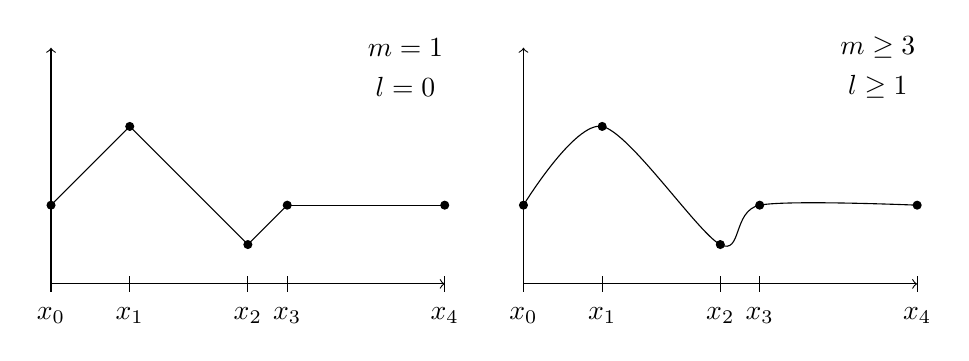
\begin{tikzpicture}
		\draw[->] (0,0) -- (5,0);
		\draw[->] (0,0) -- (0,3);
		
		\draw (0,0.1) -- (0,-0.1);
		\draw (1,0.1) -- (1,-0.1);
		\draw (2.5,0.1) -- (2.5,-0.1);
		\draw (3,0.1) -- (3,-0.1);
		\draw (5,0.1) -- (5,-0.1);
		\node at (0,-0.4) (a) {$x_0$};
		\node at (1,-0.4) (b) {$x_1$};
		\node at (2.5,-0.4) (c) {$x_2$};
		\node at (3,-0.4) (d) {$x_3$};
		\node at (5,-0.4) (e) {$x_4$};
		
		\draw[fill=black] (0,1) circle (0.05);
		\draw[fill=black] (1,2) circle (0.05);
		\draw[fill=black] (2.5,0.5) circle (0.05);
		\draw[fill=black] (3,1) circle (0.05);
		\draw[fill=black] (5,1) circle (0.05);
		\draw (0,1) -- (1,2);
		\draw (1,2) -- (2.5,0.5);
		\draw (2.5,0.5) -- (3,1);
		\draw (3,1) -- (5,1);
		
		\node at (4.5,3) (l) {$m=1$};
		\node at (4.5,2.5) (l) {$l=0$};
		
		\draw[->] (6,0) -- (11,0);
		\draw[->] (6,0) -- (6,3);
		
		\draw (6,0.1) -- (6,-0.1);
		\draw (7,0.1) -- (7,-0.1);
		\draw (8.5,0.1) -- (8.5,-0.1);
		\draw (9,0.1) -- (9,-0.1);
		\draw (11,0.1) -- (11,-0.1);
		\node at (6,-0.4) (a) {$x_0$};
		\node at (7,-0.4) (b) {$x_1$};
		\node at (8.5,-0.4) (c) {$x_2$};
		\node at (9,-0.4) (d) {$x_3$};
		\node at (11,-0.4) (e) {$x_4$};
		
		\draw[fill=black] (6,1) circle (0.05);
		\draw[fill=black] (7,2) circle (0.05);
		\draw[fill=black] (8.5,0.5) circle (0.05);
		\draw[fill=black] (9,1) circle (0.05);
		\draw[fill=black] (11,1) circle (0.05);
		\coordinate (X0) at (6,1);
		\coordinate (X1) at (7,2);
		\coordinate (X2) at (8.5,0.5);
		\coordinate (X3) at (9,1);
		\coordinate (X4) at (11,1);
		\draw[smooth] plot coordinates {(X0) (X1) (X2) (X3) (X4)};
		
		\node at (10.5,3) (l) {$m\ge 3$};
		\node at (10.5,2.5) (l) {$l\ge 1$};
	\end{tikzpicture}
\end{center}

\subsection{Interpolation durch kubische Polynomsplines}

Gegeben sei eine Zerlegung $\Delta$ und die Stützwerte $f_0,...,f_n$. Gesucht ist eine Funktion $s\in\mathcal{S}^l_3(\Delta)$ mit $l=1,2$ derart, dass
\begin{align}
	\label{1.6}
	s(x_k)=f_k\quad\text{für } k=0,...,n
\end{align}
Jede derartige Funktion heißt \begriff{kubischer Interpolationspline}.

\textbf{Konstruktion eines solchen Splines:}
\begin{align}
	h_k &:= x_{k-1}-x_k\quad\text{für } k=0,...,n-1 \notag \\
	m_k &:= s'(x_k) \quad\text{für } k=0,...,n-1\notag
\end{align}
Wegen $l\in\{1,2\}$ ist $s$ zunächst stetig differenzierbar. Wegen $s_k=s\vert_{[x_k,x_{k+1}]}$ für $k=0,...,n-1$ und $m=3$ kann man folgenden Ansatz für $s_k$ benutzen:
\begin{align}
	\label{1.7}
	s_k(x)=a_k(x-x_k)^3+b_k(x-x_k)^2+c_k(x-x_k)+d_k
\end{align}
Aus den Interpolationsbedingungen \cref{1.6} und der stetigen Differenzierbarkeit aller Funktionen in $s\in\mathcal{S}^l_m(\Delta)$ für $l\ge 1$ ergeben sich folgende Forderungen an $s_k$, $k=0,...,n-1$:
\begin{equation}
	\label{1.8}
	\begin{split}
		s_k(x_k) &= f_k \quad\text{und }\quad s_k(x_{k+1}) = f_{k+1} \\
		s'_k(x_k) &= m_k \quad\text{und }\quad s'_k(x_{k+1}) = m_{k+1}
	\end{split}
\end{equation}
Diese liefern:
\begin{equation}
	\label{1.9}
	\begin{split}
		d_k &= s_k(x_k)=f_k \\
		c_k &= s'_k(x_k)=m_k
	\end{split}
\end{equation}
und damit:
\begin{align}
	s_k(x_{k+1}) &= a_kh_k^3 + b_kh_k^2+m_kh_k + f_k = f_{k+1} \notag \\
	s'_k(x_{k+1}) &= 3a_kh_k^2 + 2b_kh_k + m_k = m_{k+1} \notag
\end{align}
Damit ergeben sich $a_k$ und $b_k$ als eindeutige Lösung für das lineare Gleichungssystem
\begin{align}
	\label{1.10}
	\begin{pmatrix}
		h_k^3 & h_k^2 \\ 3h_k^2 & 2h_k
	\end{pmatrix}
	\begin{pmatrix}
		a_k \\ b_k
	\end{pmatrix}=
	\begin{pmatrix}
		f_{k+1}-f_k-m_kf_k \\
		m_{k+1}-m_k
	\end{pmatrix}
\end{align}
Die Determinante ist $-h_k^4\neq 0$.

\begin{proposition}
	Sei eine Zerlegung $\Delta$ des Intervalls $[a,b]$ gegeben. Dann gibt es für beliebig gewählte reelle Zahlen $f_0,...,f_n$ und $m_0,...,m_n$ einen Interpolationsspline $s\in\mathcal{S}^1_3(\Delta)$, der den Interpolationsbedingungen
	\begin{align}
		s'(x_0)=m_0,...,s'(x_n)=m_n\notag
	\end{align}
	genügt. Außerdem gilt:
	\begin{align}
		s\vert_{[x_k,x_{k+1}]}=s_k\quad\text{für } k=0,...,n-1\notag
	\end{align}
	mit $s_k$ entsprechend \cref{1.7}, wobei sich $a_k,b_k,c_k,d_k$ aus \cref{1.9} und \cref{1.10} ergeben.
\end{proposition}

Für die Wahl der $m_k$ gibt es verschiedene Möglichkeiten, zum Beispiel:
\begin{itemize}
	\item Falls Ableitungswerte der zu interpolierenden Funktion $f$ bekannt sind, kann man $m_k=f'(x_k)$ setzen.
	\item Man wählt $m_0,...,m_n$ so, dass $s$ zweimal stetig differenzierbar ist, das heißt $s\in\mathcal{S}^2_3(\Delta)$ statt  $s\in\mathcal{S}^1_3(\Delta)$ gilt.
\end{itemize}

\subsection{Interpolation mit kubischen $C^2$-Splines}

Damit ein kubischer Interpolationsspline $s$ zu $\mathcal{S}^2_3(\Delta)$ gehört, muss neben den Forderungen in \cref{1.8} die Stetigkeit von $s''$ an den Stützstellen $x_1,...,x_{n-1}$ gewährleistet sein. Also hat man zusätzliche Bedingungen
\begin{align}
	s''_k(x_{k+1})=s''_{k+1}(x_{k+1})\quad\text{für } k=0,...,n-2\notag
\end{align}
Mit \cref{1.7} ergibt sich $s''(x)=6a_k(x-x_0)+2b_k$ für $x\in[x_k,x_{k+1}]$ und damit $s''_k(x_{k+1}) = 6a_kh_k+2b_k$ und $s''_{k+1}(x_{k+1})=2b_{k+1}$, also 
\begin{align}
	\label{1.11}
	3a_kh_k+b_k=b_{k+1}\quad\text{für }k=0,...,n-2
\end{align}
Aus \cref{1.10} folgt
\begin{align}
	a_k &= \frac{-2}{h_k^2}(f_{k+1}-f_k)+\frac{1}{h_k^2}(m_k+m_{k+1}) \notag \\
	b_k &= \frac{3}{h_k^2}(f_{k+1}-f_k)-\frac{1}{h_k}(2m_k+m_{k+1})\notag
\end{align}
für $k=0,...,n-1$. Wegen \cref{1.11} erhält man für $k=0,...,n-2$
\begin{align}
	& \frac{-6}{h_k^2}(f_{k+1}-f_k) + \frac{3}{h_k}(m_k+m_{k+1}) + \frac{3}{h_k^2}(f_{k+1}-f_k) - \frac{1}{h_k}(2m_k+m_{k+1}) \notag \\
	&= \frac{-6}{h^2_{k+1}}(f_{k+2}-f_{k+1})-\frac{1}{h_{k+1}}(2m_{k+1}+m_{k+2})\notag
\end{align}
Damit folgt 
\begin{align}
	\frac{1}{h_k}(m_k+2m_{k+1}) + \frac{1}{h_{k+1}}(2m_{k+1}+m_{k+2}) &= \frac{3}{h_k^2}(f_{k+1}-f_k) + \frac{3}{h_{k+1}^2}(f_{k+2}-f_{k+1})\notag \\
	\text{bzw.}\quad h_{k+1}m_k + 2(h_{k+1}+h_k)m_{k+1}+h_km_{k+2} &= \frac{3h_{k+1}}{h_k}(f_{k+1}-f_k) + \frac{3h_k}{h_{k+1}}(f_{k+2}-f_{k+1})\notag
\end{align}
Also müssen die $n+1$ Zahlen $m_0,...,m_n$ den $n-1$ Gleichungen des linearen Gleichungssystems 
\begin{align}
	\begin{pmatrix}
		\lambda_0 & 2 & \mu_0 & & & \\
		 & \lambda_1 & 2 & \mu_1 & & \\
		 & & \ddots & \ddots & \ddots & \\
		 & & & \lambda_{n-2} & 2 & \mu_{n-2}
	\end{pmatrix}
	\begin{pmatrix}
		m_0 \\ m_1 \\ \vdots \\ m_n
	\end{pmatrix}
	= \begin{pmatrix}
	 r_0 \\ r_1 \\ \vdots \\ r_{n-2}
	\end{pmatrix}\notag
\end{align}
genügen, wobei $\lambda_k,\mu_k,r_k$ durch
\begin{align}
	\lambda_k &= \frac{h_{k+1}}{h_k+h_{k+1}} \notag \\
	\mu_k &= \frac{h_k}{h_k + h_{k+1}}\notag \\
	r_k &= \frac{3h_{k+1}}{h_k(h_k+h_{k+1})}(f_{k+1}-f_k) + \frac{3h_k}{h_{k+1}(h_k+h_{k+1})}(f_{k+2} - f_{k+1})\notag
\end{align}
für $k=0,...,n-2$ gegeben sind. Die Systemmatrix und die erweiterte Systemmatrix haben den Rang $n-1$. Somit ist das Gleichungssystem lösbar, besitzt aber keine eindeutige Lösung. Um solche zu erhalten, kann man zusätzliche Bedingungen stellen, etwa
\begin{enumerate}[label=(\alph*)]
	\item \textbf{natürliche Randbedingungen:} 
	\begin{align}
		\label{1.12}
		s''(x_0) = s''(x_n)=0
	\end{align}
	Diese sind gleichbedeutend mit 
	\begin{align}
		s''_0(x_0)=6a_0(x-x_0)+2b_0=0\quad\text{und}\quad s''_{n-1}(x_n)=6a_{n-1}(x_n-x_{n-1})+2b_{n-1}=0\notag
	\end{align}
	Also folgt
	\begin{align}
		b_0=0\quad\text{und}\quad 3a_{n-1}h_{n-1} + b_{n-1}=0\notag
	\end{align}
	Nutzt man noch die Darstellung für $b_0$ sowie für $a_{n-1}$ und $b_{n-1}$, so folgt
	\begin{align}
		2m_0+m_1 = \frac{3}{h_0}(f_1-f_0) \quad\text{und}\quad m_{n-1}+2m_n=\frac{3}{h_{n-1}}(f_n-f_{n-1})\notag
	\end{align}
	Fügt man beide Gleichungen geeignet zum obigen System hinzu, erhält man ein lineares Gleichungssystem mit einer regulären trigonales Systemmatrix. Dieses kann in $\mathcal{O}(n)$ Operationen gelöst werden.
	\item \textbf{Vollständige Randbedingungen:} Sind $f'(a)$ und $f'(b)$ bekannt, dann können die zusätzlichen Bedingungen
	\begin{align}
		s'(x_0)=f'(a)\quad\text{und}\quad s'(x_n)=f'(b)
	\end{align}
	mittels $m_0=f'(a)$ und $m_n=f'(b)$ geeignet in das Gleichungssystem eingefügt werden, so dass man analog zu Fall (a) eine trigonale reguläre Systemmatrix erhält.
	\item \textbf{Periodische Spline-Interpolation:} Falls
	\begin{align}
		\label{1.14}
		f'(a)=f'(b)
	\end{align}
	und $f''(a)=f''(b)$ gilt, dann sind 
	\begin{align}
	\label{1.15}
		s'(x_0)=s'(x_n)\quad\text{und}\quad s''(x_0)=s''(x_n)
	\end{align}
	sinnvolle Randbedingungen, woraus sich zwei zusätzliche lineare Gleichungen zur Ergänzung des Gleichungssystems ableiten lassen.
	\item (nicht in der Vorlesung) \textbf{Not-in-knot Bedingung:} Es soll zusätzlich
	\begin{align}
		s'''_0(x_1)=s'''_1(x_1) \quad\text{und}\quad s'''_{n-2}(x_{n-1})=s'''_{n-1}(x_{n-1})\notag
	\end{align}
	gelten, das heißt $s$ ist auf $[x_0,x_2]$ und auf $[x_{n-2},x_n]$ ein Polynom dritten Grades. Man erhält daraus die Forderungen $a_0=a_1$ und $a_{n-2}=a_{n-1}$, woraus sich zusätzliche Gleichungen in den Variablen $m_0,m_1,m_2$ und $m_{n-2},m_{n-1},m_n$ ergeben.
\end{enumerate}

\subsection{Eine Minimaleigenschaft kubischer $C^2$-Interpolationssplines}

Durch
\begin{align}
	\skalar{f}{g}:= \int_a^b f(x)g(x)\diff x\quad\text{bzw.}\quad\Vert g\Vert_2:=\sqrt{\int_a^b g(x)^2\diff x} \quad\text{ für } f,g\in L^2[a,b]\notag
\end{align}
ist ein Skalarprodukt bzw. eine Norm in $L^2[a,b]$ definiert.

\begin{proposition}
	\proplbl{satz_1_6}
	Seien $f\in C^2[a,b]$, $\Delta$ eine Zerlegung von $[a,b]$ und $f_k:=f(x_k)$ für $k=0,...,n$. Für einen Interpolationsspline $s\in\mathcal{S}^2_3(\Delta)$, der die natürlichen, vollständigen oder periodischen Randbedingungen (bei letzteren gelte \cref{1.14}) erfüllt, gilt:
	\begin{align}
		\Vert s''\Vert^2_2 = \Vert f''\Vert_2^2 - \Vert f''-s''\Vert_2^2 \le \Vert f''\Vert_2^2
	\end{align}
\end{proposition}
\begin{proof}
	Durch Nachrechnen sieht man
	\begin{align}
		\int_a^b (f''(x))^2\diff x-\int_a^b (f''(x)-s''(x))^2\diff x = \int_a^b (s''(x))^2\diff x + 2\int_a^b (f''(x)-s''(x))s''(x)\diff x \notag
	\end{align}
	Es wird nun $J:=\int_a^b (f''(x)-s''(x))s''(x)\diff x=0$ gezeigt. Mit Hilfe partieller Integration folgt
	\begin{align}
		J=(f'(x)-s'(x))s''(x)\vert_a^b - \int_a^b (f'(x)-s'(x))s'''(x)\diff x\notag
	\end{align}
	wobei $s'''$ auf jedem Teilintervall $[x_k,x_{k+1}]$ konstant ist. Dies ergibt wegen \cref{1.6}
	\begin{align}
		\int_a^b (f'(x)-s'(x))s'''(x)\diff x &= \sum_{k=0}^{n-1} s'''(x_k+\frac{h_k}{2})\int_{x_k}^{x_{x+1}}(f'(x)-s'(x))\diff x \notag \\
		&= \sum_{k=0}^{n-1} s'''(x_k+\frac{h_k}{2})(f(x_{k+1})-s(x_{k+1})-f(x_k)+s(x_k)) \notag \\
		&= 0 \notag
	\end{align}
	und damit 
	\begin{align}
		J=(f'(x)-s'(x))s''(x)\vert_a^b = (f'(b)-s'(b))s''(b)-(f'(a)-s'(a))s''(a)\notag
	\end{align}
	Nutzt man nun noch \cref{1.12}, \cref{1.13} bzw. \cref{1.14} mit \cref{1.15}, so folgt $J=0$.
\end{proof}

\subsection{Interpolationsfehler bei kubischer $C^2$-Interpolation}

\begin{proposition}
	Seien $f\in C^2[a,b]$, $\Delta$ eine Zerlegung von $[a,b]$ und $f_k:=f(x_k)$ für $k=0,...,n$. Für einen Interpolationsspline $s\in\mathcal{S}^2_3(\Delta)$, der die natürlichen, vollständigen oder periodischen Randbedingungen (bei letzteren gelte \cref{1.14}) erfüllt, gilt:
	\begin{align}
		\Vert f-s\Vert_\infty \le \frac{1}{2}h^{\sfrac{3}{2}}\Vert f''\Vert_2\notag
	\end{align}
	wobei $h:=\max\{h_0,...,h_{n-1}\}$.
\end{proposition}
\begin{proof}
	Die Funktion $r:=f-s$ hat wegen \cref{1.6} die $n+1$ Nullstellen $x_0,...,x_n$. Der maximale Abstand benachbarter Nullstellen ist $h$. Nach dem Satz von Rolle besitzt $r'$ mindestens $n$ Nullstellen. Der Abstand zweier Nullstellen von $r'$ ist durch $2h$ nach oben beschränkt. Sei $z\in [a,b]$ so gewählt, dass $\vert r'(z)\vert=\Vert r'\Vert_\infty$. Dann gilt $\vert z-z^0\vert\le h$ für die $z$ am nächsten liegende Nullstelle $z^0$ von $r'$. O.B.d.A. sei $z^0\le z$. Mit der \person{Cauchy-Scharz}-Ungleichung folgt:
	\begin{align}
		\Vert r'\Vert_\infty^2 &= \vert r'(z)-r'(z^0)\vert^2 \notag \\
		\label{1.16}
		&= \left|\int_{z^0}^z r''(x)\cdot 1\diff x\right|^2  \\
		&\le \int_{z^0}^z r''(x)^2\diff x\cdot \int_{z^0}^z 1^2\diff x\notag \\
		&\le h\Vert r''\Vert_2^2\notag
	\end{align}
	Sei nun $y\in[a,b]$ so gewählt, dass $\vert r(y)\vert=\Vert r\\Vert_\infty$. Dann gilt $\vert y-y_0\vert\le \sfrac{h}{2}$ für die $y$ am nächsten liegende Nullstelle $y^0$ von $r$. O.B.d.A. sei $y^0\le y$. Mit \cref{1.16} ergibt sich
	\begin{align}
		\Vert r\Vert_\infty = \vert r(y)-r(y^0)\vert=\left|\int_{y^0}^y r'(x)\diff x\right|\le\max\vert r'(x)\vert\cdot \int_{y^0}^y \diff x\le \frac{1}{2}\Vert r'\Vert_\infty\le \frac{1}{2}h^{\sfrac{3}{2}}\Vert r''\Vert_2\notag
	\end{align}
	Mit \propref{satz_1_6} hat man $\Vert r''\Vert_2\le \Vert f\Vert_2$ und damit die Behauptung.
\end{proof}

\begin{remark}
	Besitzt $f$ eine höhere Glattheit, so kann die obige Fehlerschranke bezüglich der $h$-Potenz verbessert werden. Es lassen sich ferner Abschätzungen für $\Vert f'-s'\Vert_\infty$ und $\Vert f''-s''\Vert_\infty$ herleiten.
\end{remark}